% ============================================================
%  SECTION 3 — EXPERIMENTAL SETUP
% ============================================================


\begin{frame}{Theoretical Basis}
  \begin{itemize}
    \item \textbf{SIMP method \cite{Toh_2025}} \cite{sigmund2001, andreassen2011}:
          each element $e$ carries a pseudo-density $\rho_e\in[0,1]$.
          Effective stiffness:
          \[
            E_e = \rho_e^{\,p}\,E_0, \qquad p \ge 3
          \]
    \item \textbf{Objective}: minimise structural compliance (maximise
          stiffness) subject to a volume fraction constraint $f$:
          \[
            \min_{\boldsymbol{\rho}}\;
            \mathbf{F}^{\!\top}\mathbf{U}
            \quad\text{s.t.}\quad
            \frac{\sum \rho_e v_e}{V_0} \le f,
            \quad \mathbf{K}(\boldsymbol{\rho})\,\mathbf{U} = \mathbf{F}
          \]
    \item \textbf{Elastic energy stored}:
          \[
            E_{\text{in}} = \int_0^{\delta_{\max}} F(\delta)\,\dd{\delta}
          \]
          measured from force--displacement curve.
    \item Efficiency $\eta = E_{\text{out}} / E_{\text{in}}$
          captures hysteresis and dissipation losses.
  \end{itemize}
\end{frame}

\begin{frame}{Experimental Setup --- Overview}
  \centering
  % Schematic of testing platformm
    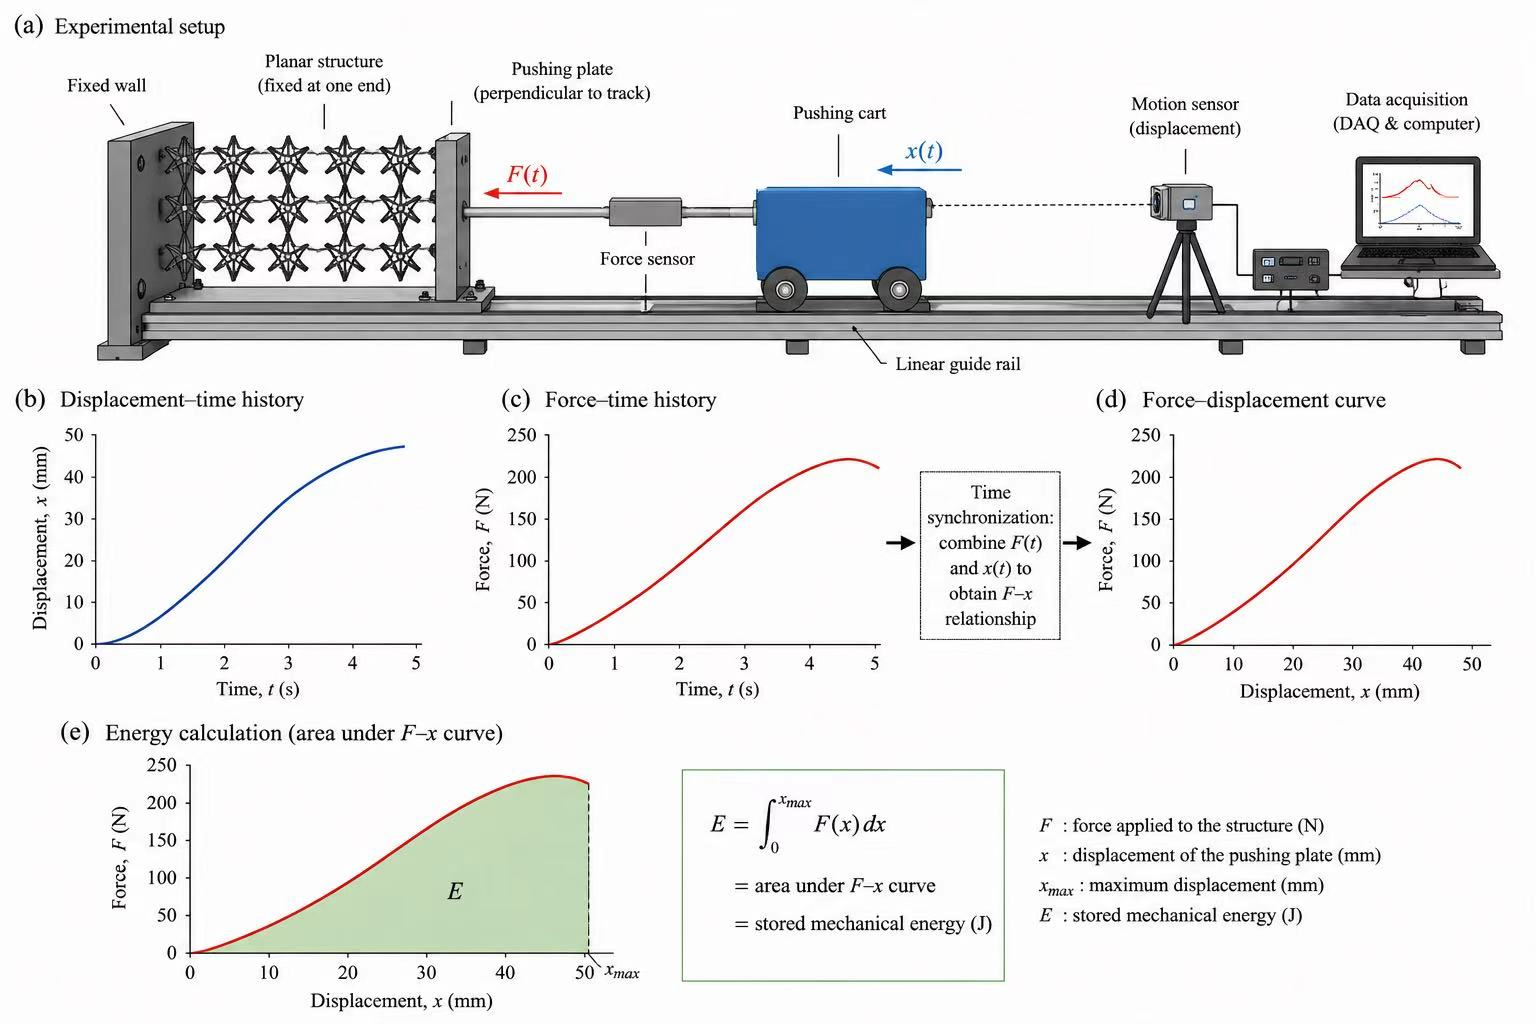
\includegraphics[width=1.05\textwidth]{figs/setup_demo.jpg}
\end{frame}

\begin{frame}{Experimental Setup --- Overview}
    \begin{itemize}
       \item \textbf{Workflow:} Quasi-static compression $\rightarrow$ Time-synced $F(t) \& x(t)$ acquisition $\rightarrow$ $F-x$ relationship transformation for energy evaluation.
        \item \textbf{Loading Method:} Quasi-static manual pushing.
        \item \textbf{Data Acquisition:} 
        \begin{itemize}
            \item Displacement $x(t)$ recorded by Motion Sensor.
            \item Applied Force $F(t)$ recorded by Force Sensor.
        \end{itemize}
        
      
        \item \textbf{Stability:} High linearity in $x(t)$ indicates steady manual loading.
    \end{itemize}
\end{frame}

\begin{frame}{Apparatus \& Materials}
  \small
  \begin{itemize}\setlength\itemsep{3pt}
    \item \textbf{Platform:} Hand wheel + lead screw compression rig (custom-built)
    \item \textbf{Force measurement:} Digital gauge, 0--50\,N, 0.1\,N resolution
    \item \textbf{Displacement:} Digital calliper, $\pm 0.01$\,mm
    \item \textbf{Material:} PLA filament (1.75\,mm), FDM 3D printing
    \item \textbf{Software:} GNU Octave, FreeCAD, Python
    \item \textbf{Environment:} Room temperature ($\sim\!25\,{}^{\circ}\mathrm{C}$)
    \item \textbf{Material:} 3D printed PETG (1.75\,mm); chosen for its superior toughness and interlayer adhesion compared to PLA, ensuring structural integrity during large deformations.
  \end{itemize}
\end{frame}

\begin{frame}{Candidate Structures}
  \centering
  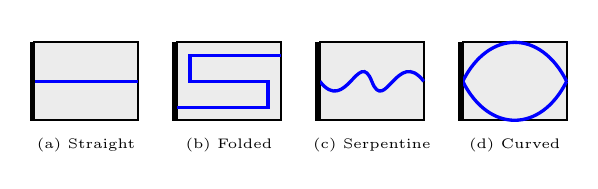
\begin{tikzpicture}[scale=0.33, every node/.style={font=\tiny}]
    % Straight beam
    \begin{scope}[xshift=0cm]
      \draw[thick, fill=gray!15] (0,0) rectangle (4,3);
      \draw[very thick, blue] (0,1.5) -- (4,1.5);
      \draw[fill=black] (-0.15,0) rectangle (0,3);
      \node[below] at (2,-0.3) {(a) Straight};
    \end{scope}

    % Folded beam
    \begin{scope}[xshift=5.5cm]
      \draw[thick, fill=gray!15] (0,0) rectangle (4,3);
      \draw[very thick, blue] (0,0.5) -- (3.5,0.5) -- (3.5,1.5)
            -- (0.5,1.5) -- (0.5,2.5) -- (4,2.5);
      \draw[fill=black] (-0.15,0) rectangle (0,3);
      \node[below] at (2,-0.3) {(b) Folded};
    \end{scope}

    % Serpentine beam
    \begin{scope}[xshift=11cm]
      \draw[thick, fill=gray!15] (0,0) rectangle (4,3);
      \draw[very thick, blue] (0,1.5)
            .. controls (1,0.2) and (1.5,2.8) .. (2,1.5)
            .. controls (2.5,0.2) and (3,2.8) .. (4,1.5);
      \draw[fill=black] (-0.15,0) rectangle (0,3);
      \node[below] at (2,-0.3) {(c) Serpentine};
    \end{scope}

    % Curved beam
    \begin{scope}[xshift=16.5cm]
      \draw[thick, fill=gray!15] (0,0) rectangle (4,3);
      \draw[very thick, blue] (0,1.5)
            .. controls (1,3.5) and (3,3.5) .. (4,1.5);
      \draw[very thick, blue] (0,1.5)
            .. controls (1,-0.5) and (3,-0.5) .. (4,1.5);
      \draw[fill=black] (-0.15,0) rectangle (0,3);
      \node[below] at (2,-0.3) {(d) Curved};
    \end{scope}
  \end{tikzpicture}

  \vspace{0.5em}
  \small
  Four manual baselines + 1--2 topology-optimised candidates.
  All share identical footprint, thickness, and boundary conditions.
  \begin{itemize}
      \item \textbf{Design space:} 4 manual baselines vs. 1--2 topology-optimized candidates.
      \item \textbf{Constraints:} Identical footprint ($W \times L$), thickness, and PETG material.
      \item \textbf{Goal:} To evaluate the influence of geometric topology on energy storage $E$.
  \end{itemize}
\end{frame}
